\section{Model-Agnostic Meta-Learning (MAML)~\cite{maml}}

\textbf{A Note: }
You may wonder why the performance of these implementations don't match the numbers reported in the original papers. One major reason is that the original papers used a different version of Omniglot few-shot classification, in which multiples of $90^{\circ}$ rotations are applied to each image to obtain 4 times the total number of images and characters. Another reason is that these implementations are designed to be pedagogical and therefore straightforward to implement from equations and pseudocode as well as trainable with minimal hyperparameter tuning. Finally, with our use of batch statistics for batch normalization during test (see code), we are technically operating in the \emph{transductive} few-shot learning setting.

\subsubsection*{MAML Algorithm Overview}

\begin{figure}[H]
\centering
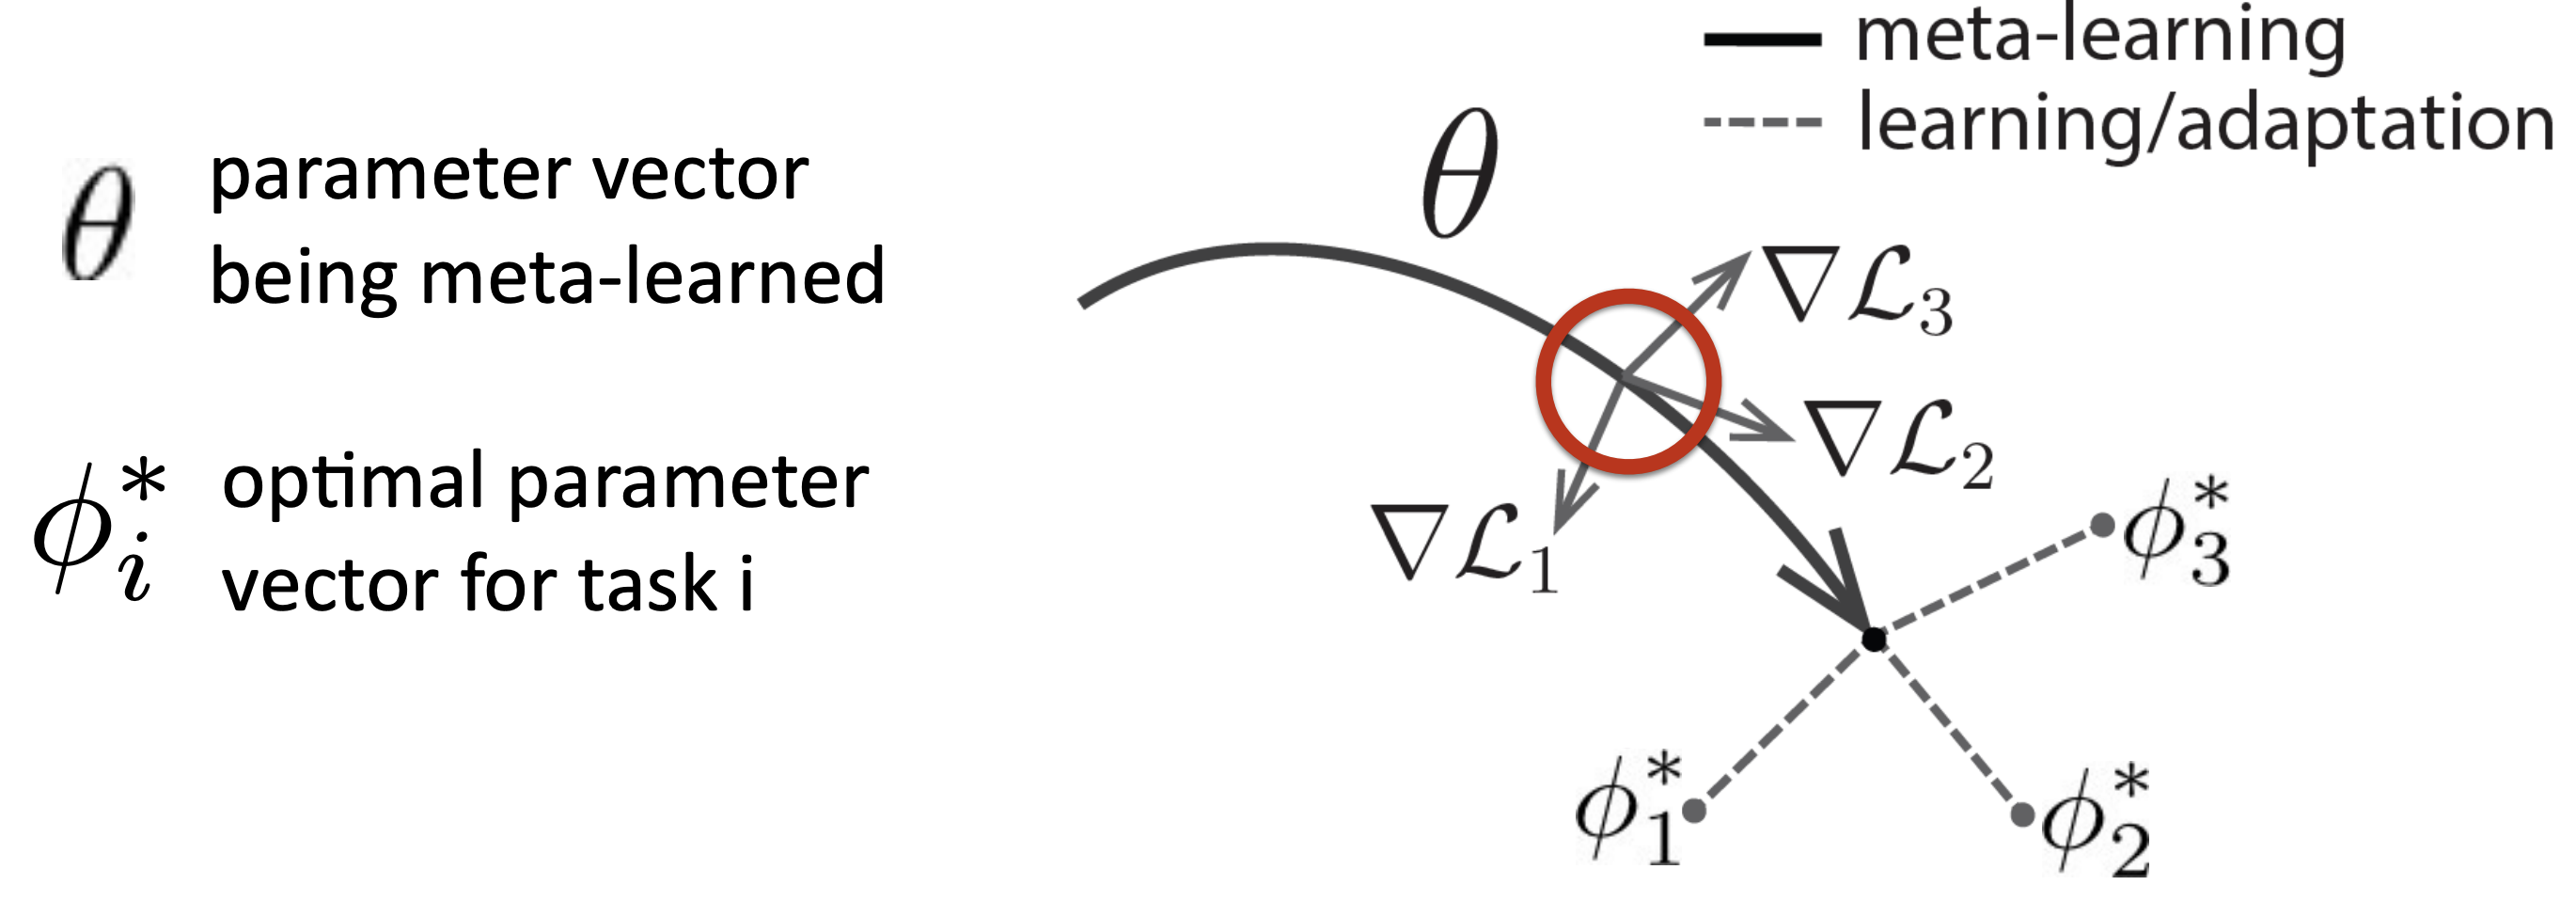
\includegraphics[width=0.8\linewidth]{./figures/MAML}
\vspace{-3mm}
\caption{MAML in a nutshell. MAML tries to find an initial parameter vector $\theta$ that can be quickly adapted via task gradients to task-specific optimal parameter vectors.}
\label{fig:maml}
\end{figure}

As discussed in lecture, the basic idea of MAML is to meta-learn parameters $\theta$ that can be quickly adapted via gradient descent to a given task. To keep notation clean, define the loss $\mathcal{L}$ of a model with parameters $\phi$ on the data $\dataset_i$ of a task $\task_i$ as
\begin{equation}\label{eq:maml loss}
    \mathcal{L}(\phi, \dataset_i) = \frac{1}{\lvert \dataset_i \rvert} \sum_{(x^j, y^j) \in \dataset_i} -\log p_\phi (y = y^j \mid x^j)
\end{equation}
Adaptation is often called the \emph{inner loop}. For a task $\task_i$ and $L$ inner loop steps, adaptation looks like the following:
\begin{equation}
\begin{aligned}
    \phi^1 &= \phi^0 - \alpha \nabla_{\phi^0} \mathcal{L}(\phi^0, \supportdata_i) \\
    \phi^2 &= \phi^1 - \alpha \nabla_{\phi^1} \mathcal{L}(\phi^1, \supportdata_i) \\
    \vdots \\
    \phi^L &= \phi^{L-1} - \alpha \nabla_{\phi^{L-1}} \mathcal{L}(\phi^{L-1}, \supportdata_i)
\end{aligned}
\end{equation}
where we have defined $\theta = \phi^0$.


Notice that only the support data is used to adapt the parameters to $\phi^L$. (In lecture, you saw $\phi^L$ denoted as $\phi_i$.) To optimize $\theta$ in the \emph{outer loop}, we use the same loss function~\eqref{eq:maml loss} applied on the adapted parameters and the query data:
\begin{equation}
    \mathcal{J}(\theta) = \E_{\task_i \sim p(\task), (\supportdata_i, \querydata_i) \sim \task_i} \left[ \mathcal{L}(\phi^L, \querydata_i) \right] \label{eq:maml_objective}
\end{equation}


For this homework, we will further consider a variant of MAML~\cite{mamlplusplus} that proposes to additionally learn the inner loop learning rates $\alpha$. Instead of a single scalar inner learning rate for all parameters, there is a separate scalar inner learning rate for each parameter group (e.g. convolutional kernel, weight matrix, or bias vector). Adaptation remains the same as in vanilla MAML except with appropriately broadcasted multiplication between the inner loop learning rates and the gradients with respect to each parameter group. 

The full MAML objective is
\begin{equation}
    \mathcal{J}(\theta, \alpha) = \E_{\task_i \sim p(\task), (\supportdata_i, \querydata_i) \sim \task_i} \left[ \mathcal{L}(\phi^L, \querydata_i) \right] \label{eq:full_objective}
\end{equation}
Like before, we will use minibatches to approximate \eqref{eq:full_objective} and use the Adam optimizer.

\begin{enumerate}[label={2.\alph*}]
    \item \points{2a} {\bf Implement Inner Loop}

In the \texttt{maml.py} file, complete the implementation of the \texttt{MAML.\_inner\_loop} which computes the task-adapted network parameters (and accuracy metrics). Pay attention to the inline comments and docstrings. \\ 
\textbf{Hint}: the simplest way to implement \texttt{\_inner\_loop} involves using \texttt{autograd.grad}.
    \item \points{2b} {\bf Implement Outer Loop}

In the \texttt{maml.py} file, complete the implementation of the \texttt{MAML.\_outer\_step} which computes the MAML objective (and more metrics). Pay attention to the inline comments and docstrings. \\
\textbf{Hint}: to understand how to use the Boolean \texttt{train} argument of \texttt{MAML.\_outer\_step}, read the documentation for the \texttt{create\_graph} argument of \texttt{autograd.grad}.

Assess your implementation of vanilla MAML on 5-way 1-shot Omniglot. 

You can run the experiment by executing: \texttt{python maml.py}

Comments from the previous part regarding arguments, checkpoints, TensorBoard, resuming training, and testing all apply. Use 1 inner loop step with a \textbf{fixed} inner learning rate of 0.4. Use 15 query examples per class per task. Do not adjust the outer learning rate from its default of $0.001$.

Your plot of the validation post-adaptation query accuracy over the course of training should look like this.
\begin{center}
    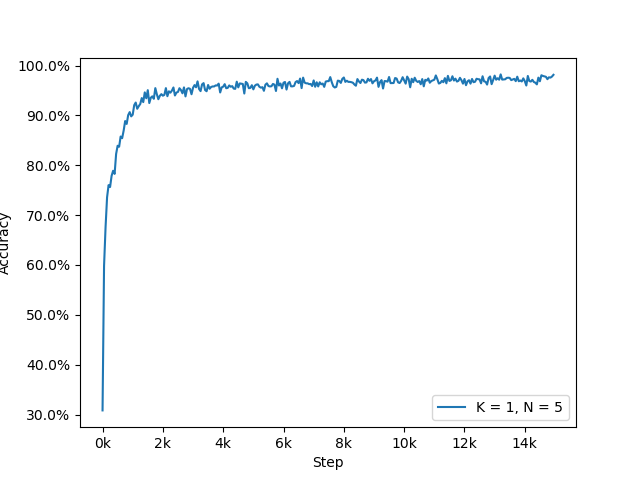
\includegraphics[width=0.75\linewidth]{./figures/maml_q1}
\end{center}

\textbf{Hint}: you should obtain a query accuracy on the validation split of at least $96\%$.


    \item \points{2c} {\bf Accuracy Metrics}

6 accuracy metrics are logged. Examine these in detail to reason about what MAML is doing.
\begin{enumerate}[label=(\roman*)]
    \item State and explain the behavior of the \texttt{train\_pre\_adapt\_support} and \texttt{val\_pre\_adapt\_support} accuracies. Your answer should explicitly refer to the task sampling process. \\ \textbf{Hint}: consult the \texttt{omniglot.py} file.

    \item Compare the \texttt{train\_pre\_adapt\_support} and \texttt{train\_post\_adapt\_support} accuracies. What does this comparison tell you about the model? Repeat for the corresponding \texttt{val} accuracies.
    
    \item Compare the \texttt{train\_post\_adapt\_support} and \texttt{train\_post\_adapt\_query} accuracies. What does this comparison tell you about the model? Repeat for the corresponding \texttt{val} accuracies.
\end{enumerate}
    \item \points{2d} {\bf Experiments - Adjusting Learning Rate and Inner Loop Steps}

\begin{enumerate}[label=(\roman*)]
    \item Try MAML with the same hyperparameters as above except for a fixed inner learning rate of $0.04$ by running \texttt{python maml.py --inner\_lr 0.04}

    Your plot of the validation post-adaptation query accuracy over the course of training with the two inner learning rates ($0.04$, $0.4$) should look as follows.
    \begin{center}
        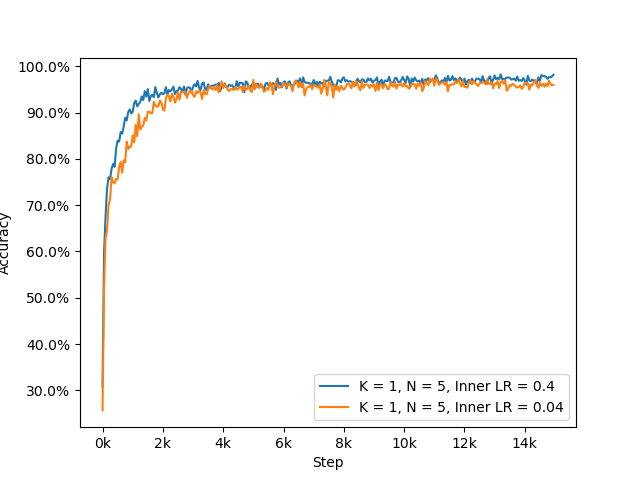
\includegraphics[width=0.75\linewidth]{./figures/maml_q3}
    \end{center}
    
    What is the effect of lowering the inner learning rate on (outer-loop) optimization and generalization?

    \item Try MAML with a fixed inner learning rate of $0.04$ for $5$ inner loop steps by \texttt{python maml.py --inner\_lr 0.04 ----num\_inner\_steps 5}

    Your plot of the validation post-adaptation query accuracy over the course of training with the two number of inner loop steps ($1$, $5$) with inner learning rate $0.04$ should look as follows.
    \begin{center}
        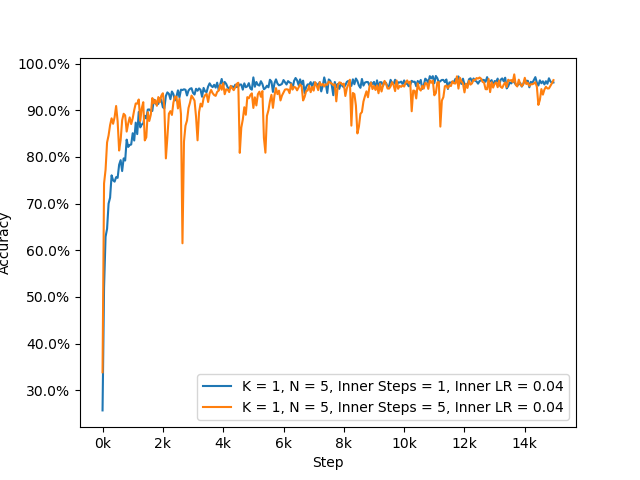
\includegraphics[width=0.75\linewidth]{./figures/maml_q4}
    \end{center}

    What is the effect of increasing the number of inner loop steps on (outer-loop) optimization and generalization?

    \item Try MAML with learning the inner learning rates by running \texttt{python maml.py --learn\_inner\_lrs}. Initialize the inner learning rates with $0.4$.

    Your plot of the validation post-adaptation query accuracy over the course of training for learning and not learning the inner learning rates, initialized at $0.4$ should look as follows.
    \begin{center}
        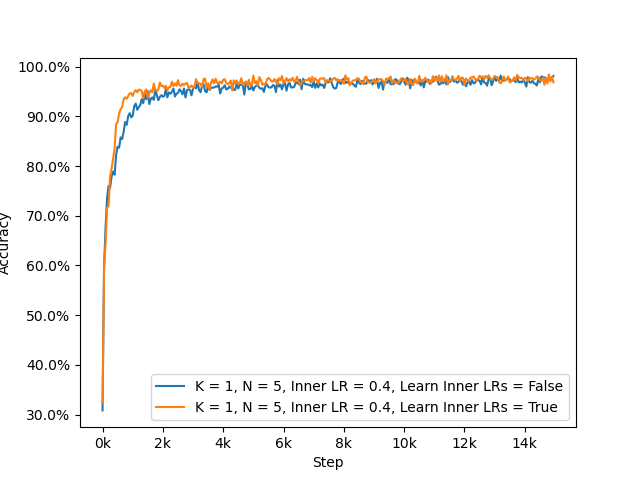
\includegraphics[width=0.75\linewidth]{./figures/maml_q5}
    \end{center}

    What is the effect of learning the inner learning rates on (outer-loop) optimization and generalization?
\end{enumerate}
\end{enumerate}

    